\begin{flushleft}
    \huge
    \textbf{3. Design}

    \Large
    \begin{enumerate}
        \item {\Large System Flow Charts} \\
            \large
            \vspace{0.2cm}
            Below is shown the Flow Chart Overview of my Entire Project. This flowchart is very abstracted without going into
            the fine detail of each Process. \\
            
            \vspace{0.5cm}
            \centerline{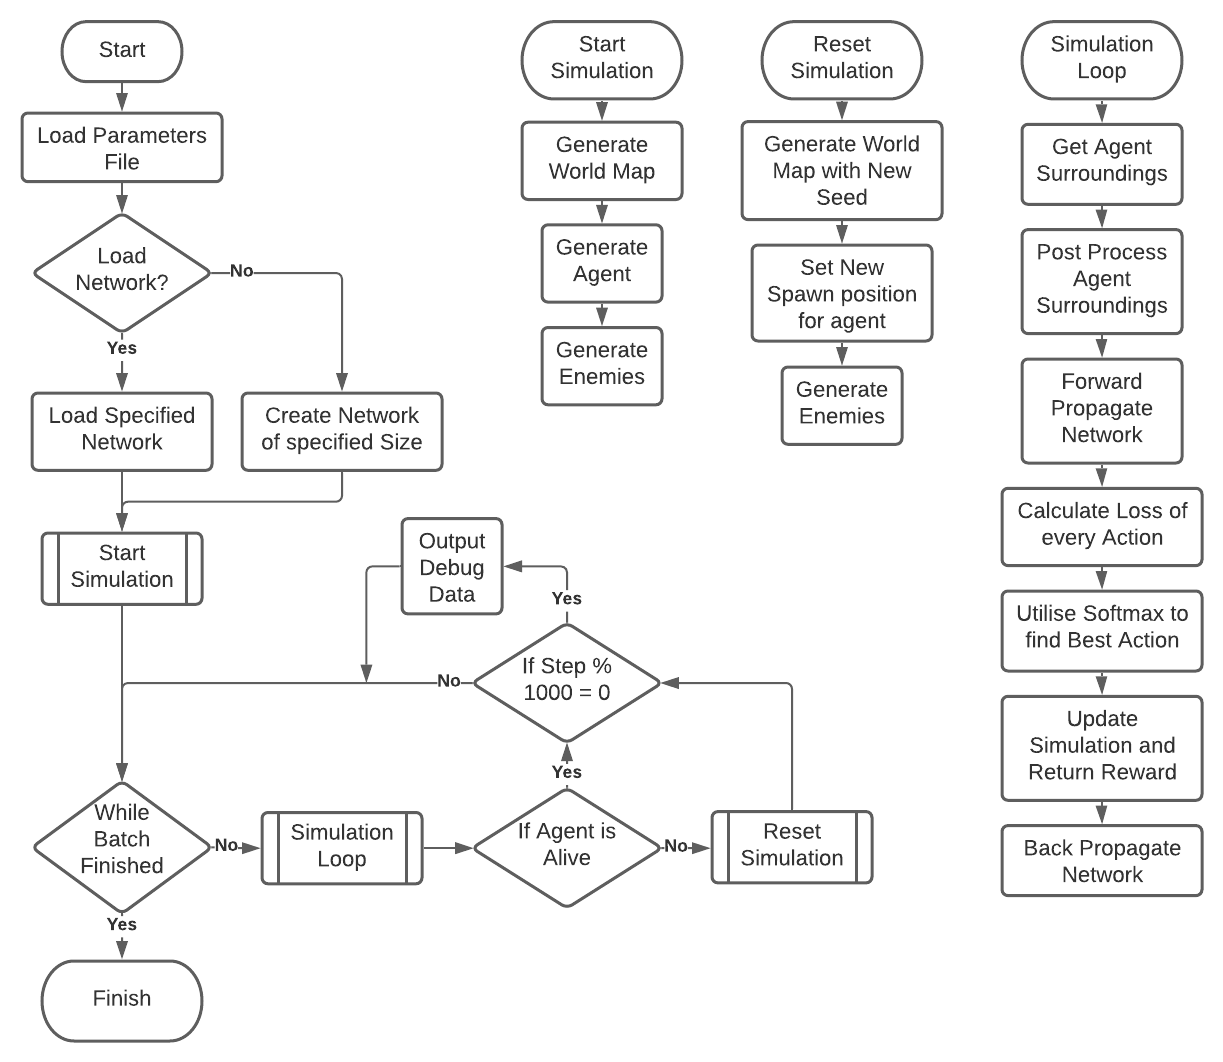
\includegraphics[width=\textwidth]{Images/Design/NEA Flow Chart.png}}
            \vspace{0.5cm}

            

        \item {\Large Class Diagrams}
            \large
            \vspace{0.2cm}

        \item {\Large Description of Algorithms}
            \large
            \vspace{0.2cm}
            \begin{enumerate}[label=\arabic*)]
                \item Matrix Addition \\
                This algorithm is a Mathematical Operation to add 2 Matrices together. To Add together 2 Matrices their Orders
                must be the same. To perform the Operation you must Sum each element in Matrix A with the corresponding element 
                in Matrix B, placing the result of each Sum in the resultant Matrix.

                \vspace{0.5cm}
                \item Matrix Subtraction \\
                This algorithm is a Mathematical Operation to subtract 2 Matrices. To Subtract 2 Matrices their Orders
                must be the same. To perform the Operation you must Sum each element in Matrix A with the negative of the 
                corresponding element in Matrix B, placing the result of each Sum in the resultant Matrix.

                \vspace{0.5cm}
                \item Matrix Multiplication \\
                This algorithm is a Mathematical Operation to find the product of 2 Matrices. To Multiply 2 Matrices
                the number of Columns in the Matrix A must be equal to the number of Rows in Matrix B. Where Matrix A has
                dimensions of $m$ x $n$ and Matrix B has dimensions of $j$ x $k$, the resultant Matrix will have dimensions of 
                $n$ x $j$. To Multiply two Matrices, the algorithm performs the Dot Product between the Row in Matrix A and the 
                corresponding Column in Matrix B. The Dot Product is the Sum of the Products of corresponding elements.

                \vspace{0.5cm}
                \item Matrix Scalar Multiplication \\
                This algorithm is a Mathematical Operation to find the product between a Matrix and a Scalar.
                The result can be found by Multiplying each element of the Matrix by the Scalar Value to form the Resultant 
                Matrix.
                
                \vspace{0.5cm}
                \item Matrix Hadamard Product \\
                This algorithm is a Mathematical Operation to another way to find the product between 2 Matrices. Instead of
                applying the Dot Product between Rows and Columns, you find the product between each element in Matrix A
                with the corresponding element in Matrix B, placing the result in the resultant Matrix. This is very epic gamer

                \vspace{0.5cm}
                \item Matrix Power \\
                This algorithm is a Mathematical Operation to find the power of a Matrix. The given Matrix needs to have square dimensions.
                The result can be found by multiplying the given Matrix by itself $n$ ammount of times where $n$ is the given power.
                
                \vspace{0.5cm}
                \item Matrix Transpose \\
                This algorithm is a Mathematical Operation used to Flip a Matrix across its Diagonal. The Transpose of any Matrix
                can be found by converting each Row of the Matrix into a Column. An $m$ x $n$ Matrix will turn into an $n$ x $m$ Matrix.
                
                \vspace{0.5cm}
                \item Activation Function Sigmoid \\
                This algorithm is a Mathematical Formulae which squishes any value to between 0 and 1. It uses Eulers Number $e$.

                \vspace{0.2cm}
                {\Large\centerline{$S(x) = \frac{1}{1 + e^{-x}}$}}
                \vspace{0.2cm}
                
                \vspace{0.5cm}
                \item Activation Function TanH \\
                This algorithm is a Hyperbolic Function which squishes any value to between -1 and 1. It is a Ratio between the two Hyperbolic 
                functions SinH and CosH. The Mathematical Formulae for this can be found under 

                \vspace{0.2cm}
                {\Large\centerline{$TanH(x) = \frac{SinH(x)}{CosH(x)} = \frac{e^x - e^{-x}}{e^x + e^{-x}}$}}
                \vspace{0.2cm}

                \vspace{0.5cm}
                \item Activation Function Relu \\
                This algorithm is a simple function which removes any negative values from its input, returning 0 instead.
                
                \vspace{0.5cm}
                \item Activation Function SoftMax \\
                This algorithm is a logistic function that creates a probability distribution from a set of points. This probability 
                distribution sums to 1. It applies the standard Exponential Function to each element, then normalises this value by dividing
                by the sum of all these Exponentials.

                \vspace{0.5cm}
                \item Neural Network Forward Propagation \\
                This algorithm is used to obtain the outputs of a Neural Network. It uses Matrix Multiplication to propagate the inputs
                of the network from Layer to Layer, eventually reaching the Output Layer. My Multiplying the Weight Matrix and the outputs
                of the previous Layer, and then adding the Bias. We can obtain the output of the layer.
                
                \vspace{0.5cm}
                \item Neural Network Loss Function \\
                The algorithm for to calculate the Loss of a Dual Neural Network can calculated by using a variation of the Bellman Equation.
                The Bellman Equation is neccesary for Mathematically Optimising in this case. It determines the Value of a decision at a certain 
                point in time, in terms of the Payoff from the Inital Action and the Value of the Potential Payoff after taking that Initial
                Action. 
                
                \vspace{0.5cm}
                \item Neural Network Backwards Propagation \\
                This algorithm is used within a Neural Network to adjust its Weights and Biases, allowing it to more accurately predict the
                best outcome. In Reinforcement Learning, the Network is trained using an estimate for what is the best action given a situation.
                Using this estimate, we can train the Network to predict this outcome by converging the series of Weights and Biases towards a
                local minimum. This is done by calculating partial derivates for every weight and bias value with respect to the cost function.
                This derivative is then subtracted from the existing weight or bias, eventually converging on the best possible value.

                \vspace{0.5cm}
                \item Agent Get Tile Vector \\
                This algorithm takes the current World Data of the simulation, and produces a Vector of Tile Data surrounding the Agent. This can
                be done using a nested For Loop rather simply.
                
                \vspace{0.5cm}
                \item Agent Post Process Tile Vector \\
                This algorithm will convert the Tile Vector into a Vector of Grayscale values, which can be used as the input for the Neural
                Network.
                
                \vspace{0.5cm}
                \item Agent Convert to Grayscale \\
                This algorithm converts a given RGB Colour Value to the corresponding Gray Scale Value. The Red, Green and Blue elements of
                the colour value are multiplied by the specific values $0.299$, $0.587$ and $0.114$. You then sum the results, and divide by 
                $255$.

                \vspace{0.5cm}
                \item Agent Spawn Position \\
                This algorithm will create a list of spawnable tiles for which the Agent could spawn on, and then randomnly select a specific
                tile as its spawn position.
                
                \vspace{0.5cm}
                \item Enemy Spawn Position \\
                This algorithm will create a list of spawnable tiles for which Enemies can spawn on, then select tiles randomnly, if they dont
                already contain an enemy or the agent it will create an Enemy Object with that position. It will do this $n$ ammount of times 
                where $n$ is the limit to how many enemies can spawn.
                
                \vspace{0.5cm}
                \item Enemy Move \\
                The algorithm I have designed for the Enemy Pathfinding is rather simple, and wont take up much runtime in my solution.
                First it calculates the distance between itself and the Agent in both Axis. The Enemy will then converge upon the Agents
                position by moving in the direction with the greatest distance, effectively finding the nearest diagonal and following it.
                The flow diagram for this Simple Algorithm is shown above under System Flow Charts.
                
                \vspace{0.5cm}
                \item Poisson Disc Sampling \\
                Poisson Disc Sampling is used to sample a set of points in N Dimensional Space. It takes two parameters, $r$ and $k$, where
                $r$ is the minimum distance a specified point must be from every other point, and $k$ is the limit of samples to choose
                before rejection. It starts by creating an N Dimensional Grid which accelerates spacial searches. An initial sample is then
                chosen and inserted into the grid. It then chooses a random point, and determines if it is greater than $r$ range from every 
                other point in the grid. This can easily be acomplished using the previously defined Grid. If after $k$ attempts, no point is
                found then the search is concluded.
                
                \vspace{0.5cm}
                \item Perlin Noise \\
                Perlin Noise is a method of generating a procedural texture depending upon input parameters. It defines an n-dimensional
                grid of Vectors, each grid intersection contains a fixed, random unit vector. To sample Perlin Noise, the grid cell which
                the point lies in must be found. The Vectors between the sampled point, and the corners of the cell. We then take the Dot
                Product between these new Vectors, and the Vectors applied to the intersections. In 2d Space this leaves us with 4 Values.
                We then use an Interpolation function to Interpolate between the 4 Values. 
                
                \vspace{0.5cm}
                \item Octave Perlin Noise \\
                Octave Perlin Noise takes the existing Perlin Noise algorithm, but adds rescaled clones of itself into itself, to create
                what is known as Fractal Noise. Creating this Fractal Noise is common practice because it reduces the sharp edges encountered
                with just the regular Perlin Noise Algorithm.

                \vspace{0.5cm}
            \end{enumerate}

        \item {\Large Description of Data Structures} \\
            \large
            \vspace{0.2cm}
            \begin{enumerate}
                \item {\large Matrices} \\
                As part of developing a Neural Network, I will extensively use Matrices, as they are an integral part of the algorithms
                used for Machine Learning. After creating a prototype Matrix class as part of my prototype, I will represent it in the
                same format. In my prototype I created a Class, and then represented the values of the Matrix with a 2d List (List of Lists).
                As part of my Matrix Class I will have multiple constructors, to help avoid repeating code.
            \end{enumerate}
            

    \end{enumerate}
    \vspace{0.1cm}
\end{flushleft}